% !TeX encoding = UTF-8

\documentclass{protokol}

\usepackage{pdfpages}
\usepackage{tikz}
\usetikzlibrary{calc}
\usetikzlibrary{arrows}

%====== Units =====
\usepackage{siunitx}
\sisetup{inter-unit-product =\ensuremath{\cdot}}
\sisetup{group-digits = integer}
\sisetup{output-decimal-marker = {,}}
\sisetup{exponent-product = \ensuremath{\cdot}}
\sisetup{separate-uncertainty}
\sisetup{tight-spacing = false}
%\sisetup{scientific-notation = true}
%\sisetup{round-mode=places,round-precision=4}
%\sisetup{evaluate-expression}


%====== Grafy =====
\usepackage{pgfplots}
\pgfplotsset{width=0.8\linewidth, compat=1.17}
\def\plotcscale{0.8}
\usepackage{pgfplotstable}
\usepackage[figurename=Obr.]{caption} % figure caption rename

%====== Rovnice align block ======
\usepackage{amsmath}
\setlength{\jot}{10pt} % rozestup mezi řádky

\graphicspath{ {./img/} }

%====== Vyplňte údaje ======
\jmeno{Jakub Charvot}
\kod{240844}
\rocnik{3.}
\obor{MET}
\skupina{MET/2}
\spolupracoval{Radek Kučera}

\merenodne{02.04.\ 2024}
\odevzdanodne{09.04.\ 2024}
\nazev{Měření veličin pomocí polohového MEMS senzoru}
\cislo{10} %měřené úlohy

\predmet{Mikrosenzory a mikromechanické systémy}
\ustav{Ústav mikroelektroniky}
\skola{FEKT VUT v~Brně}

\def\para{x+0}
\def\parb{\para-80}


% %citace 
% \usepackage[backend=biber, style=iso-numeric, sortlocale=cs_CZ, autolang=other, language=czech]{biblatex}
% \addbibresource{bibliography.bib}
% \DeclareFieldFormat{labelnumberwidth}{\mkbibbrackets{#1}}
% hyperlinky
\usepackage[colorlinks]{hyperref}

% odstavce
\usepackage{parskip}

% Bloky kódu
\usepackage{xcolor}

%New colors defined below
\definecolor{codegreen}{rgb}{0,0.6,0}
\definecolor{codegray}{rgb}{0.5,0.5,0.5}
\definecolor{codepurple}{rgb}{0.58,0,0.82}
\definecolor{backcolour}{rgb}{0.95,0.95,0.92}

\usepackage{listings}
\lstdefinestyle{mystyle}{
  backgroundcolor=\color{backcolour}, commentstyle=\color{codegreen},
  keywordstyle=\color{magenta},
  numberstyle=\tiny\color{codegray},
  stringstyle=\color{codepurple},
  basicstyle=\ttfamily\footnotesize,
  breakatwhitespace=false,         
  breaklines=true,                 
  captionpos=b,                    
  keepspaces=true,                 
  numbers=left,                    
  numbersep=5pt,                  
  showspaces=false,                
  showstringspaces=false,
  showtabs=false,                  
  tabsize=2
}
\lstset{
	inputencoding=utf8,
	extendedchars=true,
	literate={á}{{\'a}}1 {č}{{\v{c}}}1 {ď}{{\v{d}}}1 {é}{{\'e}}1 {ě}{{\v{e}}}1 
           {í}{{\'i}}1 {ň}{{\v{n}}}1 {ó}{{\'o}}1 {ř}{{\v{r}}}1 {š}{{\v{s}}}1 
           {ť}{{\v{t}}}1 {ú}{{\'u}}1 {ů}{{\r{u}}}1 {ý}{{\'y}}1 {ž}{{\v{z}}}1 
           {Á}{{\'A}}1 {Č}{{\v{C}}}1 {Ď}{{\v{D}}}1 {É}{{\'E}}1 {Ě}{{\v{E}}}1 
           {Í}{{\'I}}1 {Ň}{{\v{N}}}1 {Ó}{{\'O}}1 {Ř}{{\v{R}}}1 {Š}{{\v{S}}}1 
           {Ť}{{\v{T}}}1 {Ú}{{\'U}}1 {Ů}{{\r{U}}}1 {Ý}{{\'Y}}1 {Ž}{{\v{Z}}}1,
	style=mystyle
	}

    \lstset{
    language=Python,  % Specify the language for syntax highlighting
    basicstyle=\small\ttfamily,  % Set the basic style for the code
    keywordstyle=\color{blue},  % Set style for keywords
    commentstyle=\color{green!50!black},  % Set style for comments
    stringstyle=\color{orange},  % Set style for strings
    showstringspaces=false,  % Do not show spaces in strings
    breaklines=true,  % Enable line wrapping
    tabsize=4  % Set tab size
}

% Číslování
\pagenumbering{arabic}

% Tabulky
\usepackage{booktabs}

% =========================================
% =============== DOKUMENT ================
% =========================================
\begin{document}
	%====== Vygenerování tabulky ======a
    \maketitle

    \section{Měření a jeho vyhodnocení }
        Maximální absolutní chyba použitého senzoru je \(\pm \qty{0.22}{\degree}\), což je údaj platný jak pro měření rotace, tak i náklonu -- jedná se o stále stejný typ měření, pouze využívá jinou osu senzoru. 

        \begin{table}[ht!]
            \caption{Nastavené a měřené hodnoty (ADXL345).}
            \def\arraystretch{1.2}
            \centering
            \begin{tabular}{rrrrr}
\toprule
$\theta_{rot-nast}\ [^\circ]$ & $\theta_{rot-mer}\ [^\circ]$ & $\Delta \theta_{rot} \ [^\circ]$ & $\theta_{nak-nast}\ [^\circ]$ & $\theta_{nak-mer}\ [^\circ]$ \\
\midrule
90,000 & 87,138 & 2,047 & 90,000 & 87,953 \\
80,000 & 77,793 & 1,171 & 80,000 & 78,829 \\
70,000 & 67,770 & 0,715 & 70,000 & 69,285 \\
60,000 & 57,801 & 0,563 & 60,000 & 59,437 \\
50,000 & 48,346 & 0,184 & 50,000 & 49,816 \\
40,000 & 38,345 & 0,037 & 40,000 & 39,963 \\
30,000 & 28,879 & -0,346 & 30,000 & 30,346 \\
20,000 & 18,929 & 0,019 & 20,000 & 19,981 \\
10,000 & 9,645 & -1,123 & 10,000 & 11,123 \\
0,000 & -0,448 & -1,560 & 0,000 & 1,560 \\
-10,000 & -11,354 & -0,831 & -10,000 & -9,169 \\
-20,000 & -21,389 & -0,575 & -20,000 & -19,425 \\
-30,000 & -30,961 & -0,509 & -30,000 & -29,491 \\
-40,000 & -39,973 & -1,043 & -40,000 & -38,957 \\
-50,000 & -50,243 & -0,828 & -50,000 & -49,172 \\
-60,000 & -59,785 & -1,243 & -60,000 & -58,757 \\
-70,000 & -70,255 & -1,390 & -70,000 & -68,610 \\
-80,000 & -79,226 & -1,078 & -80,000 & -78,922 \\
-90,000 & -88,276 & -1,904 & -90,000 & -88,096 \\
\bottomrule
\end{tabular}

        \end{table}

    \begin{figure}[h!]
        \centering
        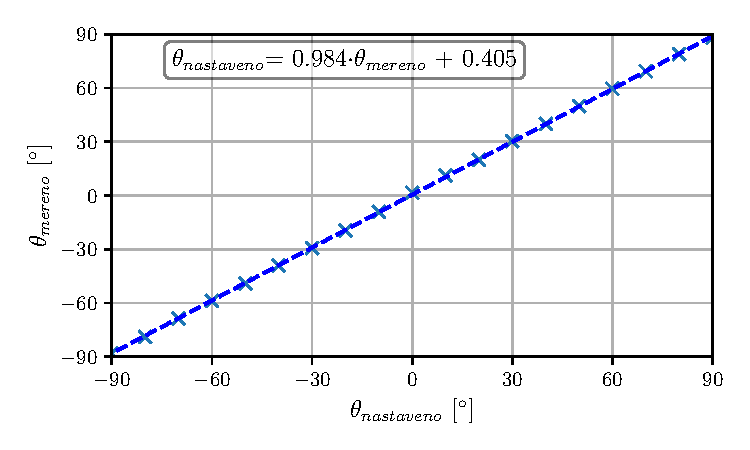
\includegraphics[width=0.8\textwidth]{img/naklon-kalib.pdf}
        \caption{Kalibrační křivka měření náklonu.}
        \label{fig:img/graf-1}
    \end{figure}
    
    \begin{figure}[h!]
        \centering
        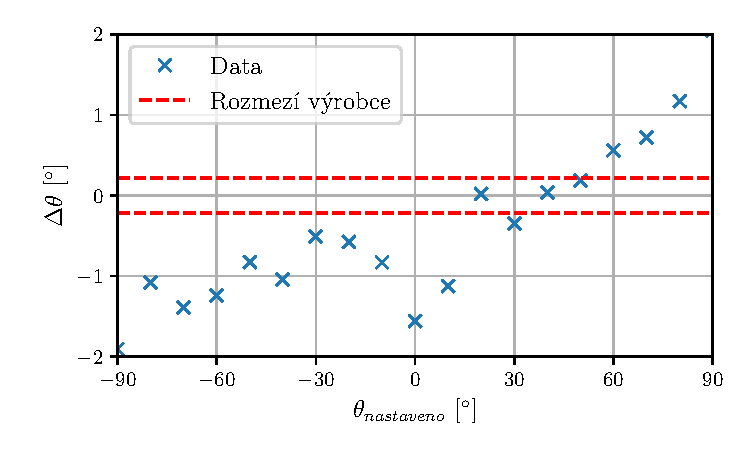
\includegraphics[width=0.8\textwidth]{img/naklon-korek.pdf}
        \caption{Korekční křivka měření náklonu.}
        \label{fig:img/graf-1}
    \end{figure}

    \begin{figure}[h!]
        \centering
        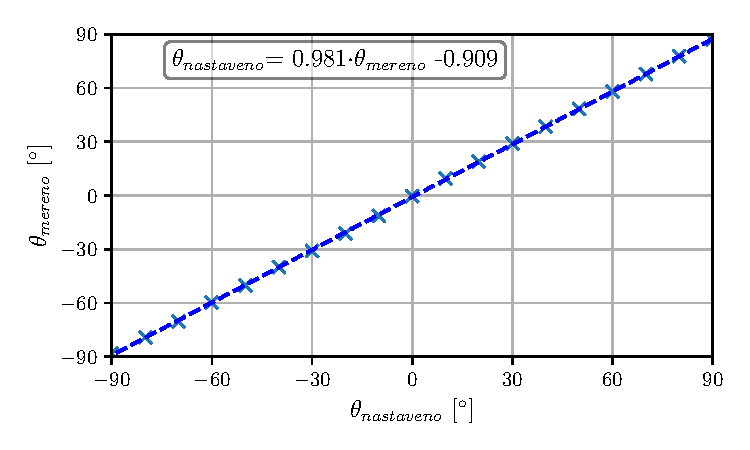
\includegraphics[width=0.8\textwidth]{img/rotace-kalib.pdf}
        \caption{Kalibrační křivka měření rotace.}
        \label{fig:img/graf-2}
    \end{figure}

    \begin{figure}[h!]
        \centering
        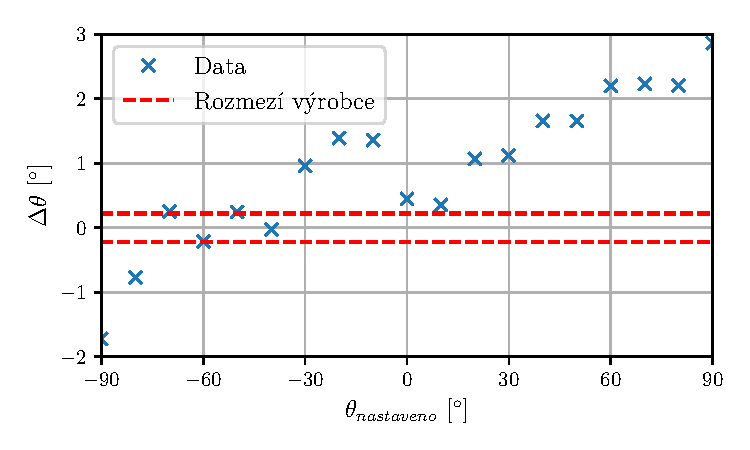
\includegraphics[width=0.8\textwidth]{img/rotace-korek.pdf}
        \caption{Korekční křivka měření rotace.}
        \label{fig:img/graf-2}
    \end{figure}

    \subsubsection{Příklad výpočtu}
    
    \[
        \Delta \theta_{rot} = \theta_{rot-nast} - \theta_{rot-mer} \\
        \Delta \theta_{nak} = \theta_{nak-nast} - \theta_{nak-mer} 
    \]

    \clearpage
    \subsection{Zdrojový kód}
    \lstinputlisting[caption={Použitý kód v jazyce Python}, label=lst:example]{data/_code.py}

    \begin{table}[ht!]
        \caption{Měřené a vypočtené hodnoty (ADXL203).}
        \def\arraystretch{1.2}
        \centering
        \begin{tabular}{|c|c|c|c|c|c|}
            \hline \multicolumn{3}{|c|}{ Vibrace v ose X } & \multicolumn{3}{|c|}{ Vibrace v ose Y } \\
            \hline $\mathrm{f}_{\mathrm{Hz}}[\mathrm{Hz}]$ & \begin{tabular}{c} 
            Amplituda \\
            {$[-]$}
            \end{tabular} & \begin{tabular}{c}
            $\mathrm{f}_{\mathrm{RPM}}$ \\
            {$[\mathrm{RPM}]$}
            \end{tabular} & $\mathrm{f}_{\mathrm{Hz}}[\mathrm{Hz}]$ & \begin{tabular}{c} 
            Amplituda \\
            {$[-]$}
            \end{tabular} & \begin{tabular}{c}
            $\mathrm{f}_{\mathrm{RPM}}$ \\
            {$[\mathrm{RPM}]$}
            \end{tabular} \\
            \hline \multicolumn{6}{|c|}{$\mathrm{U}=4,5 \mathrm{~V}$} \\
            \hline 777 & 0,034 &  & 483 & 0,013 & \\
            \hline 678 & 0,009 &      & 387 & 0,017 & \\
            \hline 488 & 0,009 &      & 309 & 0,021 & \\
            \hline 387 & 0,0106 & 23220 & 195 & 0,035 & 11700 \\
            \hline \multicolumn{6}{|c|}{$\mathrm{U}=6 \mathrm{~V}$} \\
            \hline 762 & 0,06 &   & 286 & 0,015 &  \\
            \hline 503 & 0,017 &      & 251 & 0,012 & \\
            \hline 375 & 0,013 &      & 218 & 0,019 & 13080 \\
            \hline 285 & 0,012 & 17100  & 926 & 0,031 &  \\
            \hline \multicolumn{6}{|c|}{$\mathrm{U}=8 \mathrm{~V}$} \\
            \hline 802 & 0,052 &  & 450 & 0,022 &  \\
            \hline 767 & 0,022 &      & 314 & 0,016 & \\
            \hline 602 & 0,024 &      & 285 & 0,028 & \\
            \hline 280 & 0,037 & 16800  & 161 & 0,031 & 9660 \\
            \hline \multicolumn{6}{|c|}{$\mathrm{U}=10 \mathrm{~V}$} \\
            \hline 777 & 0,101 &  & 549 & 0,0222 &  \\
            \hline 554 & 0,025 &      & 342 & 0,016 & \\
            \hline 336 & 0,044 &      & 192 & 0,028 & \\
            \hline 240 & 0,037 & 14400  & 139 & 0,031 & 8340 \\
            \hline \multicolumn{6}{|c|}{$\mathrm{U}=12 \mathrm{~V}$} \\
            \hline 625 & 0,0394 & & 324 & 0,069 &  \\
            \hline 217 & 0,062 &      & 275 & 0,058 & \\
            \hline 754 & 0,065 &      & 166 & 0,055 & \\
            \hline 53  & 0,133 & 3180  & 86  & 0,045 & 5160 \\
            \hline
            \end{tabular}
    
    \end{table}

        
        \clearpage
        \section*{Závěr}
            V této úloze jsme za pomoci předpřipraveného Python kódu pracovali se dvěmi typy akcelerometrů. V první části jsme využili schopnost senzoru měřit statické zrychlení ve třech osách. Při náklonu senzoru se mění rozložení tíhové síly mezi osami a lze tedy vypočítat úhel náklonu. Z přiložených kalibračních křivek vyplývá, že senzor měří poměrně přesně a lineárně v celém svém rozsahu, absolutní chyba nikdy nepřesahuje \qty{2}{\degree}, ovšem výrobce garantuje hodnotu ještě o řád menší a tento požadavek rozhodně splněn není.  Jelikož program automaticky přepočítává měřenou analogovou hodnotu na údaj náklonu de stupních a k původní hodnotě nemáme přístup, nemá zde smysl mluvit o citlivosti senzoru, i když to po nás zadání vyžaduje. 

            Ve druhé části úlohy jsme měřili dynamické zrychlení, v našem případě vibrace. Kvůli naprosto nevhodnému způsobu zpracování dat, který autor úlohy zvolil (i přesto, že měl k dispozici plné možnosti jazyka Python a mohl využít algoritmicky mnohem přesnější metodu) jsou námi získaná data zatížena velkou chybou. Hodnotu základní frekvence ze které se má dále počítat rychlost otáček se nám podařilo zachytit pouze v několika případech a tedy ani vypočtené hodnoty neodpovídají předpokládanému trendu. 
\end{document}
